% Options for packages loaded elsewhere
\PassOptionsToPackage{unicode}{hyperref}
\PassOptionsToPackage{hyphens}{url}
%
\documentclass[
  man]{apa6}
\usepackage{amsmath,amssymb}
\usepackage{iftex}
\ifPDFTeX
  \usepackage[T1]{fontenc}
  \usepackage[utf8]{inputenc}
  \usepackage{textcomp} % provide euro and other symbols
\else % if luatex or xetex
  \usepackage{unicode-math} % this also loads fontspec
  \defaultfontfeatures{Scale=MatchLowercase}
  \defaultfontfeatures[\rmfamily]{Ligatures=TeX,Scale=1}
\fi
\usepackage{lmodern}
\ifPDFTeX\else
  % xetex/luatex font selection
\fi
% Use upquote if available, for straight quotes in verbatim environments
\IfFileExists{upquote.sty}{\usepackage{upquote}}{}
\IfFileExists{microtype.sty}{% use microtype if available
  \usepackage[]{microtype}
  \UseMicrotypeSet[protrusion]{basicmath} % disable protrusion for tt fonts
}{}
\makeatletter
\@ifundefined{KOMAClassName}{% if non-KOMA class
  \IfFileExists{parskip.sty}{%
    \usepackage{parskip}
  }{% else
    \setlength{\parindent}{0pt}
    \setlength{\parskip}{6pt plus 2pt minus 1pt}}
}{% if KOMA class
  \KOMAoptions{parskip=half}}
\makeatother
\usepackage{xcolor}
\usepackage{graphicx}
\makeatletter
\def\maxwidth{\ifdim\Gin@nat@width>\linewidth\linewidth\else\Gin@nat@width\fi}
\def\maxheight{\ifdim\Gin@nat@height>\textheight\textheight\else\Gin@nat@height\fi}
\makeatother
% Scale images if necessary, so that they will not overflow the page
% margins by default, and it is still possible to overwrite the defaults
% using explicit options in \includegraphics[width, height, ...]{}
\setkeys{Gin}{width=\maxwidth,height=\maxheight,keepaspectratio}
% Set default figure placement to htbp
\makeatletter
\def\fps@figure{htbp}
\makeatother
\setlength{\emergencystretch}{3em} % prevent overfull lines
\providecommand{\tightlist}{%
  \setlength{\itemsep}{0pt}\setlength{\parskip}{0pt}}
\setcounter{secnumdepth}{-\maxdimen} % remove section numbering
% Make \paragraph and \subparagraph free-standing
\makeatletter
\ifx\paragraph\undefined\else
  \let\oldparagraph\paragraph
  \renewcommand{\paragraph}{
    \@ifstar
      \xxxParagraphStar
      \xxxParagraphNoStar
  }
  \newcommand{\xxxParagraphStar}[1]{\oldparagraph*{#1}\mbox{}}
  \newcommand{\xxxParagraphNoStar}[1]{\oldparagraph{#1}\mbox{}}
\fi
\ifx\subparagraph\undefined\else
  \let\oldsubparagraph\subparagraph
  \renewcommand{\subparagraph}{
    \@ifstar
      \xxxSubParagraphStar
      \xxxSubParagraphNoStar
  }
  \newcommand{\xxxSubParagraphStar}[1]{\oldsubparagraph*{#1}\mbox{}}
  \newcommand{\xxxSubParagraphNoStar}[1]{\oldsubparagraph{#1}\mbox{}}
\fi
\makeatother
% definitions for citeproc citations
\NewDocumentCommand\citeproctext{}{}
\NewDocumentCommand\citeproc{mm}{%
  \begingroup\def\citeproctext{#2}\cite{#1}\endgroup}
\makeatletter
 % allow citations to break across lines
 \let\@cite@ofmt\@firstofone
 % avoid brackets around text for \cite:
 \def\@biblabel#1{}
 \def\@cite#1#2{{#1\if@tempswa , #2\fi}}
\makeatother
\newlength{\cslhangindent}
\setlength{\cslhangindent}{1.5em}
\newlength{\csllabelwidth}
\setlength{\csllabelwidth}{3em}
\newenvironment{CSLReferences}[2] % #1 hanging-indent, #2 entry-spacing
 {\begin{list}{}{%
  \setlength{\itemindent}{0pt}
  \setlength{\leftmargin}{0pt}
  \setlength{\parsep}{0pt}
  % turn on hanging indent if param 1 is 1
  \ifodd #1
   \setlength{\leftmargin}{\cslhangindent}
   \setlength{\itemindent}{-1\cslhangindent}
  \fi
  % set entry spacing
  \setlength{\itemsep}{#2\baselineskip}}}
 {\end{list}}
\usepackage{calc}
\newcommand{\CSLBlock}[1]{\hfill\break\parbox[t]{\linewidth}{\strut\ignorespaces#1\strut}}
\newcommand{\CSLLeftMargin}[1]{\parbox[t]{\csllabelwidth}{\strut#1\strut}}
\newcommand{\CSLRightInline}[1]{\parbox[t]{\linewidth - \csllabelwidth}{\strut#1\strut}}
\newcommand{\CSLIndent}[1]{\hspace{\cslhangindent}#1}
\ifLuaTeX
\usepackage[bidi=basic]{babel}
\else
\usepackage[bidi=default]{babel}
\fi
\babelprovide[main,import]{english}
% get rid of language-specific shorthands (see #6817):
\let\LanguageShortHands\languageshorthands
\def\languageshorthands#1{}
% Manuscript styling
\usepackage{upgreek}
\captionsetup{font=singlespacing,justification=justified}

% Table formatting
\usepackage{longtable}
\usepackage{lscape}
% \usepackage[counterclockwise]{rotating}   % Landscape page setup for large tables
\usepackage{multirow}		% Table styling
\usepackage{tabularx}		% Control Column width
\usepackage[flushleft]{threeparttable}	% Allows for three part tables with a specified notes section
\usepackage{threeparttablex}            % Lets threeparttable work with longtable

% Create new environments so endfloat can handle them
% \newenvironment{ltable}
%   {\begin{landscape}\centering\begin{threeparttable}}
%   {\end{threeparttable}\end{landscape}}
\newenvironment{lltable}{\begin{landscape}\centering\begin{ThreePartTable}}{\end{ThreePartTable}\end{landscape}}

% Enables adjusting longtable caption width to table width
% Solution found at http://golatex.de/longtable-mit-caption-so-breit-wie-die-tabelle-t15767.html
\makeatletter
\newcommand\LastLTentrywidth{1em}
\newlength\longtablewidth
\setlength{\longtablewidth}{1in}
\newcommand{\getlongtablewidth}{\begingroup \ifcsname LT@\roman{LT@tables}\endcsname \global\longtablewidth=0pt \renewcommand{\LT@entry}[2]{\global\advance\longtablewidth by ##2\relax\gdef\LastLTentrywidth{##2}}\@nameuse{LT@\roman{LT@tables}} \fi \endgroup}

% \setlength{\parindent}{0.5in}
% \setlength{\parskip}{0pt plus 0pt minus 0pt}

% Overwrite redefinition of paragraph and subparagraph by the default LaTeX template
% See https://github.com/crsh/papaja/issues/292
\makeatletter
\renewcommand{\paragraph}{\@startsection{paragraph}{4}{\parindent}%
  {0\baselineskip \@plus 0.2ex \@minus 0.2ex}%
  {-1em}%
  {\normalfont\normalsize\bfseries\itshape\typesectitle}}

\renewcommand{\subparagraph}[1]{\@startsection{subparagraph}{5}{1em}%
  {0\baselineskip \@plus 0.2ex \@minus 0.2ex}%
  {-\z@\relax}%
  {\normalfont\normalsize\itshape\hspace{\parindent}{#1}\textit{\addperi}}{\relax}}
\makeatother

\makeatletter
\usepackage{etoolbox}
\patchcmd{\maketitle}
  {\section{\normalfont\normalsize\abstractname}}
  {\section*{\normalfont\normalsize\abstractname}}
  {}{\typeout{Failed to patch abstract.}}
\patchcmd{\maketitle}
  {\section{\protect\normalfont{\@title}}}
  {\section*{\protect\normalfont{\@title}}}
  {}{\typeout{Failed to patch title.}}
\makeatother

\usepackage{xpatch}
\makeatletter
\xapptocmd\appendix
  {\xapptocmd\section
    {\addcontentsline{toc}{section}{\appendixname\ifoneappendix\else~\theappendix\fi: #1}}
    {}{\InnerPatchFailed}%
  }
{}{\PatchFailed}
\makeatother
\keywords{MovieLens, demographics, data visualization, consumer behavior, genres\newline\indent Word count: X}
\DeclareDelayedFloatFlavor{ThreePartTable}{table}
\DeclareDelayedFloatFlavor{lltable}{table}
\DeclareDelayedFloatFlavor*{longtable}{table}
\makeatletter
\renewcommand{\efloat@iwrite}[1]{\immediate\expandafter\protected@write\csname efloat@post#1\endcsname{}}
\makeatother
\usepackage{lineno}

\linenumbers
\usepackage{csquotes}
\ifLuaTeX
  \usepackage{selnolig}  % disable illegal ligatures
\fi
\usepackage{bookmark}
\IfFileExists{xurl.sty}{\usepackage{xurl}}{} % add URL line breaks if available
\urlstyle{same}
\hypersetup{
  pdftitle={Demographic Insights on Film Ratings and Preferences},
  pdfauthor={First Author1},
  pdflang={en-EN},
  pdfkeywords={MovieLens, demographics, data visualization, consumer behavior, genres},
  hidelinks,
  pdfcreator={LaTeX via pandoc}}

\title{Demographic Insights on Film Ratings and Preferences}
\author{First Author\textsuperscript{1}}
\date{}


\shorttitle{Film Preferences by Demographics}

\authornote{

The authors acknowledge the support of the GroupLens Research Project for making the MovieLens dataset publicly available. We also thank the R community for providing robust data visualization tools.

The authors made the following contributions. First Author: Conceptualization, Writing - Original Draft Preparation, Writing - Review \& Editing.

Correspondence concerning this article should be addressed to First Author, Postal address. E-mail: \href{mailto:my@email.com}{\nolinkurl{my@email.com}}

}

\affiliation{\vspace{0.5cm}\textsuperscript{1} Wilhelm-Wundt-University}

\abstract{%
Consumer preferences in entertainment can be strongly influenced by demographic factors. Using the MovieLens 100k dataset, we examined how age, gender, and occupation shape movie ratings and genre preferences. The results suggest that younger viewers may gravitate more toward action and sci-fi, while older viewers show higher ratings for dramas and romances. Occupation groups also displayed unique genre affinities. These insights can inform recommendation algorithms, marketing strategies, and content creation to cater to distinct audience segments. Future work should consider additional demographic dimensions and more contemporary datasets.
}



\begin{document}
\maketitle

\section{Introduction}\label{introduction}

Understanding how demographic factors (e.g., age, gender, occupation) influence consumer preferences is critical for tailoring content in film recommendation systems. Past research suggests that demographic attributes can shape the types of media people enjoy and how they evaluate them (\textbf{lamovie?}; \textbf{tidyverse?}).

\textbf{Research Questions:}

\begin{enumerate}
\def\labelenumi{\arabic{enumi}.}
\item
  \textbf{Primary Question:} How do demographic factors---particularly age, gender, and occupation---influence movie ratings and genre preferences?
\item
  \textbf{Secondary Questions:}

  \begin{itemize}
  \tightlist
  \item
    Do younger vs.~older users differ significantly in their average ratings and preferred genres?
  \item
    Are there distinct genre preferences when comparing male vs.~female viewers?
  \item
    How do occupational groups differ in their rating patterns?
  \end{itemize}
\end{enumerate}

We hypothesize that younger viewers will rate action and sci-fi genres more favorably, while older viewers will show a preference for drama and romance. We also expect subtle differences between genders and distinct patterns across occupations.

\section{Method}\label{method}

\subsection{Data Source and Collection}\label{data-source-and-collection}

We used the \textbf{MovieLens 100k dataset}, collected by the GroupLens Research Project at the University of Minnesota (September 1997--April 1998) (\textbf{movielens?}). Users of the MovieLens platform voluntarily rated movies on a 1--5 scale. Demographic details (age, gender, occupation, zip code) were self-reported. The dataset includes 100,000 ratings from 943 users on 1,682 movies.

\subsection{Participants}\label{participants}

\begin{itemize}
\tightlist
\item
  \textbf{Users (N=943):} Each user rated at least 20 movies.
\item
  \textbf{Demographics:} Mean age \textasciitilde{} 34 years, gender recorded as M/F, and a wide range of occupations (e.g., student, educator, technician).
\end{itemize}

\subsection{Materials (Data)}\label{materials-data}

\begin{itemize}
\tightlist
\item
  \textbf{Ratings Data (u.data):} \texttt{user\_id}, \texttt{movie\_id}, \texttt{rating}, \texttt{timestamp}.
\item
  \textbf{User Data (u.user):} \texttt{user\_id}, \texttt{age}, \texttt{gender}, \texttt{occupation}, \texttt{zip\_code}.
\item
  \textbf{Item Data (u.item):} \texttt{movie\_id}, \texttt{title}, \texttt{release\_date}, genres (19 binary indicators).
\end{itemize}

\subsection{Procedure}\label{procedure}

The data was obtained from the MovieLens website, where users rated movies voluntarily. We merged all three data files into one comprehensive dataset.

\subsection{Data Analysis}\label{data-analysis}

All analyses were conducted in R using the \texttt{tidyverse} for data wrangling and \texttt{ggplot2} for visualization (\textbf{tidyverse?}). We used papaja for APA-formatting.

\section{Results}\label{results}

\subsection{Descriptive Statistics}\label{descriptive-statistics}

\begin{verbatim}
## # A tibble: 2 x 4
##   gender mean_rating sd_rating     n
##   <chr>        <dbl>     <dbl> <int>
## 1 F             3.53      1.17 25740
## 2 M             3.53      1.11 74260
\end{verbatim}

\emph{Interpretation}: Both male and female viewers have similar average ratings, though small differences may emerge when we look at genres.

\subsection{Visualization 1: Average Ratings by Age Group for a Selected Genre}\label{visualization-1-average-ratings-by-age-group-for-a-selected-genre}

We first examine how ratings differ by age group for the ``Fantasy'' genre as an example. Here we create age groups and visualize the differences.

\begin{figure}
\centering
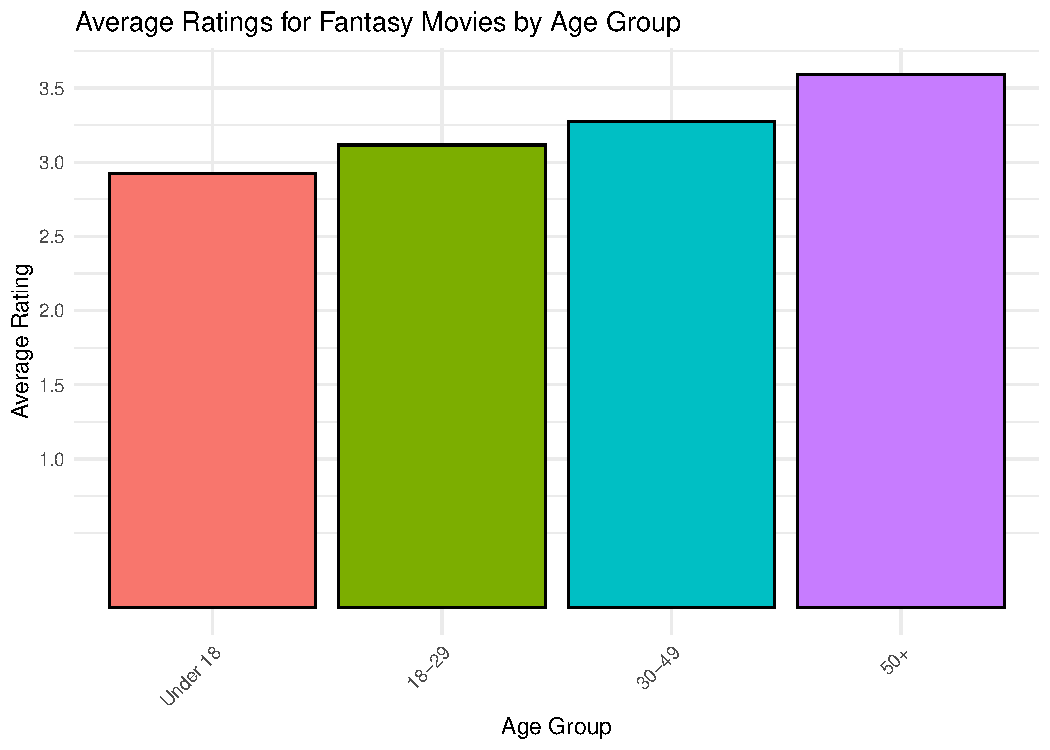
\includegraphics{Project_files/figure-latex/age-groups-plot-1.pdf}
\caption{\label{fig:age-groups-plot}Average Ratings for Fantasy Movies by Age Group}
\end{figure}

\emph{Interpretation:} There may be slight variations in how different age groups rate fantasy films, with younger viewers showing slightly different patterns compared to older ones.

\subsection{Visualization 2: Genre Preferences by Gender}\label{visualization-2-genre-preferences-by-gender}

We now look at a more complex visualization: average ratings for a selection of popular genres by gender. We will visualize multiple genres in a single plot.

\begin{figure}
\centering
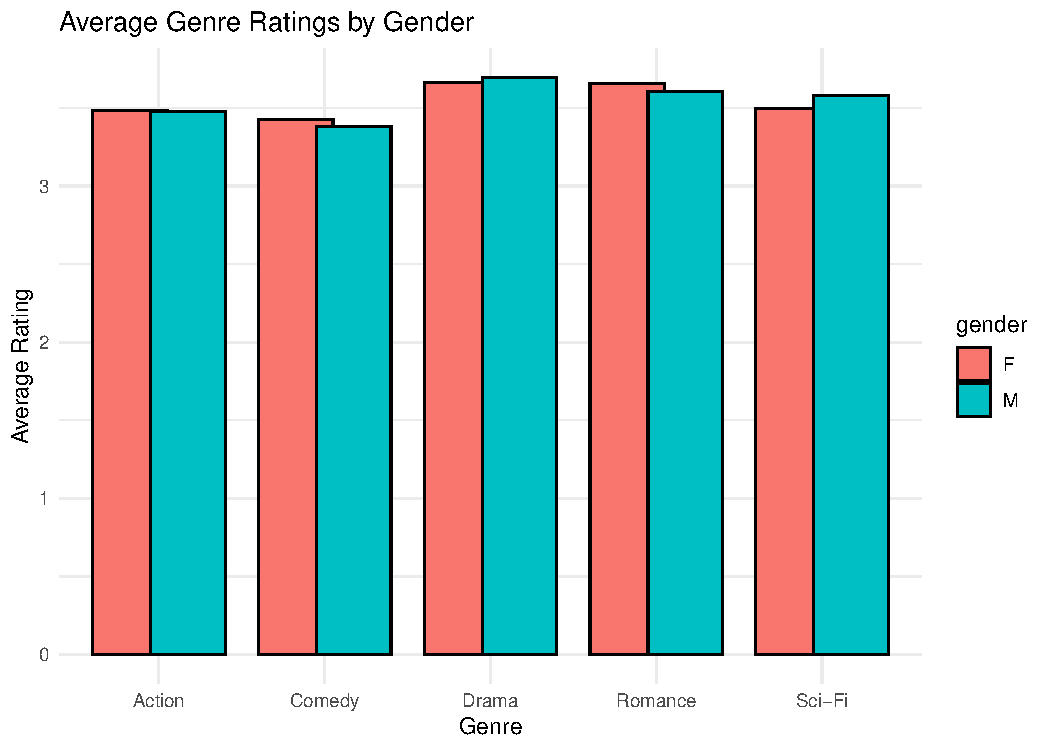
\includegraphics{Project_files/figure-latex/genre-gender-plot-1.pdf}
\caption{\label{fig:genre-gender-plot}Average Genre Ratings by Gender}
\end{figure}

\emph{Interpretation:} Differences emerge by gender for certain genres. For example, one gender may show a slightly higher affinity for Romance than another.

\subsection{Table: Top 5 Genres by Occupation (Mean Ratings)}\label{table-top-5-genres-by-occupation-mean-ratings}

Instead of a third plot, we include a table summarizing how different occupations rate the top five genres (by overall average rating in that occupation group).

\begin{verbatim}
## # A tibble: 105 x 4
## # Groups:   occupation [21]
##    occupation    genre       mean_rating     n
##    <chr>         <chr>             <dbl> <int>
##  1 administrator Film-Noir          3.97   147
##  2 administrator War                3.92   786
##  3 administrator Documentary        3.88    48
##  4 administrator Drama              3.80  3099
##  5 administrator Mystery            3.76   385
##  6 artist        Film-Noir          4.23    64
##  7 artist        Documentary        4.15    34
##  8 artist        War                3.90   225
##  9 artist        Western            3.86    29
## 10 artist        Sci-Fi             3.82   308
## # i 95 more rows
\end{verbatim}

\emph{Interpretation:} Occupations differ in their top-rated genres, indicating that profession-related cultural factors may influence movie preferences.

\subsection{Answering the Research Questions}\label{answering-the-research-questions}

\begin{itemize}
\tightlist
\item
  \textbf{Age Differences:} Preliminary evidence suggests younger viewers might rate certain genres (like Fantasy) differently than older viewers.\\
\item
  \textbf{Gender Differences:} Some genres show small but noticeable differences in average ratings between males and females.\\
\item
  \textbf{Occupation Differences:} Occupation categories differ in their top 5 genres, hinting at profession-based preference clusters.
\end{itemize}

Overall, demographic variables do influence how films are rated and which genres are favored.

\section{Discussion}\label{discussion}

The results indicate demographic factors are intertwined with movie rating behaviors. Age-group differences in genre preferences support the idea that generational cohorts have distinct cinematic tastes. Gender-based differences, while subtle, may reflect societal stereotypes or cultural norms around certain genres. Occupational differences could stem from varying educational backgrounds, interests, and lifestyle patterns.

These findings have practical implications for recommendation systems, which can be improved by factoring in demographic information. Marketers and content creators can target specific demographic groups more effectively, tailoring film releases or promotional campaigns.

\textbf{Limitations} include the dataset's temporal constraints (late 1990s) and binary gender classification. Future research should integrate more recent datasets, non-binary gender identifications, and geographic or cultural variables for a more comprehensive understanding.

\section{References}\label{references}

\phantomsection\label{refs}
\begin{CSLReferences}{0}{1}
\end{CSLReferences}

```

\begin{center}\rule{0.5\linewidth}{0.5pt}\end{center}


\end{document}
